\documentclass{standalone}

\usepackage{tikz}
\usetikzlibrary{calc}

\begin{document}
  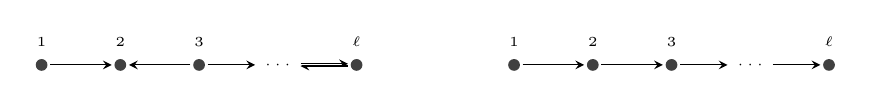
\begin{tikzpicture}
    \tikzstyle{v1} = [color=darkgray, circle, outer sep=1pt, fill, inner
      sep=1.5pt]
    \tikzstyle{v2} = [color=darkgray, circle, outer sep=1pt, fill, inner
      sep=3.0pt]
    \tikzstyle{e} = [->, >={stealth}] \tikzset{font=\tiny}

    \begin{scope}
      \node[v1, label={1}] (1) at (0,0) {};
      \node[v1, label={2}] (2) at (1,0) {};
      \node[v1, label={3}] (3) at (2,0) {};
      \node (mid) at (3,0) {$\cdots$};
      \node[v1, label={$\ell$}] (4) at (4,0) {};
      \draw[e] (1) -- (2);
      \draw[e] (3) -- (2);
      \draw[e] (3) -- (mid);

      % This is far too complicated for the effect I want.
      \begin{scope}[transform canvas = {yshift = \pgflinewidth}]
        \clip ($ (4) - (0,0.3\pgflinewidth) $) rectangle (2,2);
        \draw[e] (mid) -- (4);
      \end{scope}
      \begin{scope}[transform canvas = {yshift = -\pgflinewidth}]
        \clip ($ (4) + (0,0.3\pgflinewidth) $) rectangle (2,-2);
        \draw[e] (4) -- (mid);
      \end{scope}
    \end{scope}

    \begin{scope}[shift={(6,0)}]
      \node[v1, label={1}] (1) at (0,0) {};
      \node[v1, label={2}] (2) at (1,0) {};
      \node[v1, label={3}] (3) at (2,0) {};
      \node (mid) at (3,0) {$\cdots$};
      \node[v1, label={$\ell$}] (4) at (4,0) {};
      \draw[e] (1) -- (2);
      \draw[e] (2) -- (3);
      \draw[e] (3) -- (mid);
      \draw[e] (mid) -- (4);
    \end{scope}

  \end{tikzpicture}
\end{document}
